\begin{figure}[h!]
\tikzset{every picture/.style={line width=0.75pt}} %set default line width to 0.75pt        
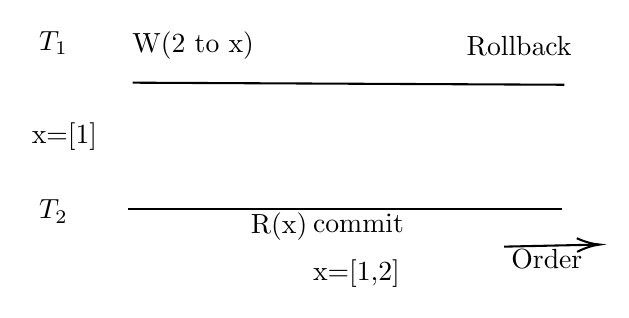
\begin{tikzpicture}[x=0.75pt,y=0.75pt,yscale=-1,xscale=1]
%uncomment if require: \path (0,300); %set diagram left start at 0, and has height of 300

%Straight Lines [id:da9500410641573396] 
\draw    (62.56,29) -- (270.56,30) ;
%Straight Lines [id:da7796185686481738] 
\draw    (60.56,90) -- (269.56,90) ;
%Straight Lines [id:da7329480179958066] 
\draw    (241.56,108) -- (285.56,107.04) ;
\draw [shift={(287.56,107)}, rotate = 178.75] [color={rgb, 255:red, 0; green, 0; blue, 0 }  ][line width=0.75]    (10.93,-3.29) .. controls (6.95,-1.4) and (3.31,-0.3) .. (0,0) .. controls (3.31,0.3) and (6.95,1.4) .. (10.93,3.29)   ;

% Text Node
\draw (16,3) node [anchor=north west][inner sep=0.75pt]   [align=left] {$T_1$};
% Text Node
\draw (16,84) node [anchor=north west][inner sep=0.75pt]   [align=left] {$T_2$};
% Text Node
\draw (61,3) node [anchor=north west][inner sep=0.75pt]   [align=left] {W(2 to x)};
% Text Node
\draw (118,90) node [anchor=north west][inner sep=0.75pt]   [align=left] {R(x)};
% Text Node
\draw (222,5) node [anchor=north west][inner sep=0.75pt]   [align=left] {Rollback};
% Text Node
\draw (148,91) node [anchor=north west][inner sep=0.75pt]   [align=left] {commit};
% Text Node
\draw (243.56,108) node [anchor=north west][inner sep=0.75pt]   [align=left] {Order};
% Text Node
\draw (12.5,47) node [anchor=north west][inner sep=0.75pt]   [align=left] {x=[1]};
% Text Node
\draw (148,113) node [anchor=north west][inner sep=0.75pt]   [align=left] {x=[1,2]};

\end{tikzpicture}
\caption{P1: Dirty Read between $T_1$ and $T_2$}
\end{figure}